\documentclass[a4paper, 11pt]{article}
\usepackage[french]{babel}
\usepackage[utf8]{inputenc}
\usepackage[T1]{fontenc}
\usepackage{datetime}
\usepackage{float}
\usepackage{eurosym}
\usepackage{comment} % enables the use of multi-line comments (\ifx \fi)
\usepackage{graphicx}

\usepackage{fullpage} % changes the margin
\begin{document}
%Header-Make sure you update this information!!!!
\noindent
\large\textbf{Cahier des charges} \hfill \textbf{Distribution de l'eau en Haïti} \\
\normalsize Deknop Céline \hfill Université catholique de Louvain \\
Hallet Adrien \hfill \today \\
Strebelle Sébastien

\section*{Abstract}
Cahier des charges du projet de gestion de distribution d'eau en Haïti, mémoire UCLouvain 2018-2019. Destiné aux intervenants du projet et contenant les propositions pour la future application.
\hrule
\section{Glossaire}
% Liste exhaustive de tous les termes pouvant prêter à confusion
  \begin{description} %ToDo : trouver un moyen de display ça beau, je sais pas si c'est l'idéal. Aussi y'a pas moyen d'auto-sort par ordre alphabétique ?
    %ToDo 2 : définir les termes
    %ToDo 3 : ordonner alphabétiquement le truc si on peut pas le faire automatiquement
    %ToDo 4 : check le document régulièrement et ajouter tous les termes qui peuvent prêter à confusion
    \item[CAEPA]
    \item[DINEPA]
    \item[HTG]
    \item[Utilisateur]
    \item[Application ou système]
    \item[Permission]
    \item[éléments du réseau de distribution de type "sortie"] %TODO change in text
    \item[Profils]
    \item[Client]
    \item[Citizen science]
    \item[Réseau]
    \item[Fontaine]
    \item[Kiosque]
    \item[Réservoir]
    \item[Prise individuelle]
  \end{description}
\section{Introduction}
% Contexte de l'application
Dans chaque section du document, nous avons ajouté une partie "Questions et remarques", où nous demandons à Protos ou aux intervenant Haïtiens de donner des précisions ou leur avis car nous estimons n'avoir pas assez d'informations ou de connaissances sur le sujet. Ce sont les points sur lesquels nous avons le plus besoin d'aide et dont il faut discuter en priorité, mais toute remarque venant des clients sera prise en compte et appréciée.
\section{Types d'utilisateurs}
Cette section du document contient une description détaillée de tous les types d'utilisateurs qui, à terme, interagiront avec l'application. Nous détaillons aussi ce que ceux-ci pourront faire avec l'application, pour vous donner un contexte familier.

  \begin{description}
    \item[Gestionnaire de fontaines] est un utilisateur auquel on assigne un ou plusieurs éléments du réseau de distribution de type "sortie" (fontaine, kiosque, réservoir, branchement individuel) dont il est responsable.
    Il gère également la gestion des consommateurs d'eau dans sa zone et les ajoute/supprime/modifie dans le système lorsque c'est nécessaire (naissance, décès, déménagement).
    Il utilise l'application pour signaler des problèmes et ainsi pouvoir en avertir le technicien/plombier et sa hiérarchie. Chaque mois, le gestionnaire de fontaines utilise l'application pour déposer un rapport. Ce rapport contient, pour chaque élément du réseau sous sa responsabilité, les quantités d'eau distribuées (si un compteur est présent), les recettes (HTG), l'état (en service, hors service). Une section générale (une seule fois par rapport) déclare également les heures et jours de service du gestionnaire de fontaines.

    \emph{Exemple : une personne chargée de gérer un point d'eau pourrait être un gestionnaire de fontaine. Il peut ainsi utiliser l'application pour envoyer mensuellement les données, ajouter les utilisateurs lorsque nécessaire et déclarer les problèmes.}

    \item[Gestionnaire de zone] est un utilisateur qui gère un groupe de gestionnaires de fontaines. Il dispose des mêmes permissions que les gestionnaires de fontaines dans sa zone et peut donc effectuer les mêmes actions avec l'application. En plus de ça, le gestionnaire de zone peut créer des profils de gestionnaires de fontaines et de techniciens/plombiers et leur assigner des permissions sur les éléments du réseau. %Meh

    \emph{Exemple 1 : Protos ou la DINEPA peuvent être assignés en tant que gestionnaires de zone ayant les accès sur tous les systèmes et agir en tant que gestionnaires généraux de tout le système. Ils peuvent donc consulter toutes les informations rapportées par les autres utilisateurs.}

    \emph{Exemple 2 : un CAEPA pourrait être assigné en tant que gestionnaire de zone et avoir accès aux infrastructures du réseau de distribution dans sa zone géographique et ainsi consulter les informations et les modifier pour venir en aide aux gestionnaires de fontaine.}

    \item[Consommateur] est un utilisateur du réseau de distribution d'eau, mais dans un premier temps, n'aura pas accès à l'application. Dans le futur, l'additiond d'un volet \emph{Citizen science} lui permettra de signaler un problème sur le réseau, de consulter l'état de celui-ci et éventuellement d'autres fonctionnalités, qui seront détaillées par la suite.

    \item[Technicien/Plombier] est un utilisateur auquel on assigne des éléments du réseau de distribution (fontaine, réservoir, prise individuelle, etc). Chaque technicien/plombier utilise l'application pour voir les problèmes déclarés par les autres utilisateurs (gestionnaires de fontaine, de zone ou consommateurs quand le volet \emph{Citizen science} sera ajouté). Il peut utiliser l'application pour répondre aux demandes d'intervention pour demander plus d'informations ou proposer une solution si le déplacement n'est pas nécessaire. Il peut modifier l'état d'un problème, demander des précisions et le marquer en cours de résolution ou résolu une fois l'intervention terminée.

    \emph{Exemple : un technicien plombier démarrant sa journée peut consulter l'application et voir quels sont les problèmes qui requièrent son attention. Il peut dialoguer avec les gestionnaires et modifier l'état des problèmes afin qu'à terme le réseau fonctionne sans problème.}

  \end{description}
  \subsection{Questions et remarques}
  % Questions
  \begin{itemize}
    \item Le contenu du rapport mensuel d'un gestionaire de fontaine sera un élément essentiel de l'application. S'il manque quoique ce soit, précisez-le nous au plus vite.
    \item Un gestionnaire de zone dont la zone recouvre tous les systèmes peut être vu comme un administrateur et aurait dès lors accès en lecture et écriture à toutes les données de l'application. Par erreur ou malveillance, il pourrait en effacer ou modifier certaines, faussant l'ensemble. Une pratique courante en informatique pour gérer ce problème potentiel est d'archiver les données : elles ne sont ainsi jamais vraiment modifiées ou effacées et peuvent être restaurées à l'état précédent. Est-ce une fonctionnalité que vous souhaitez pour l'application, ou n'est-ce pas nécéssaire de s'en occuper ? Si ce modèle d'archivage ne vous convient pas, souhaitez-vous autre chose ?
    \item L'utilisateur "technicien/plombier" et les fonctionnalités qui lui seront associées sont une interprétation de notre part car il nous semblait pratique de pouvoir centraliser la gestion du réseau de distribution entièrement au sein de l'application. Cela vous semble-t-il utile d'avoir une interface destinée au technicien ?
  \end{itemize}

\section{Fonctionnalités}
% Liste exhaustive des fonctionnalités de l'application
  \subsection{Questions et remarques}
\section{Exemples principaux}
  \subsection{Fonctionnement général}
    \begin{figure}[H]
        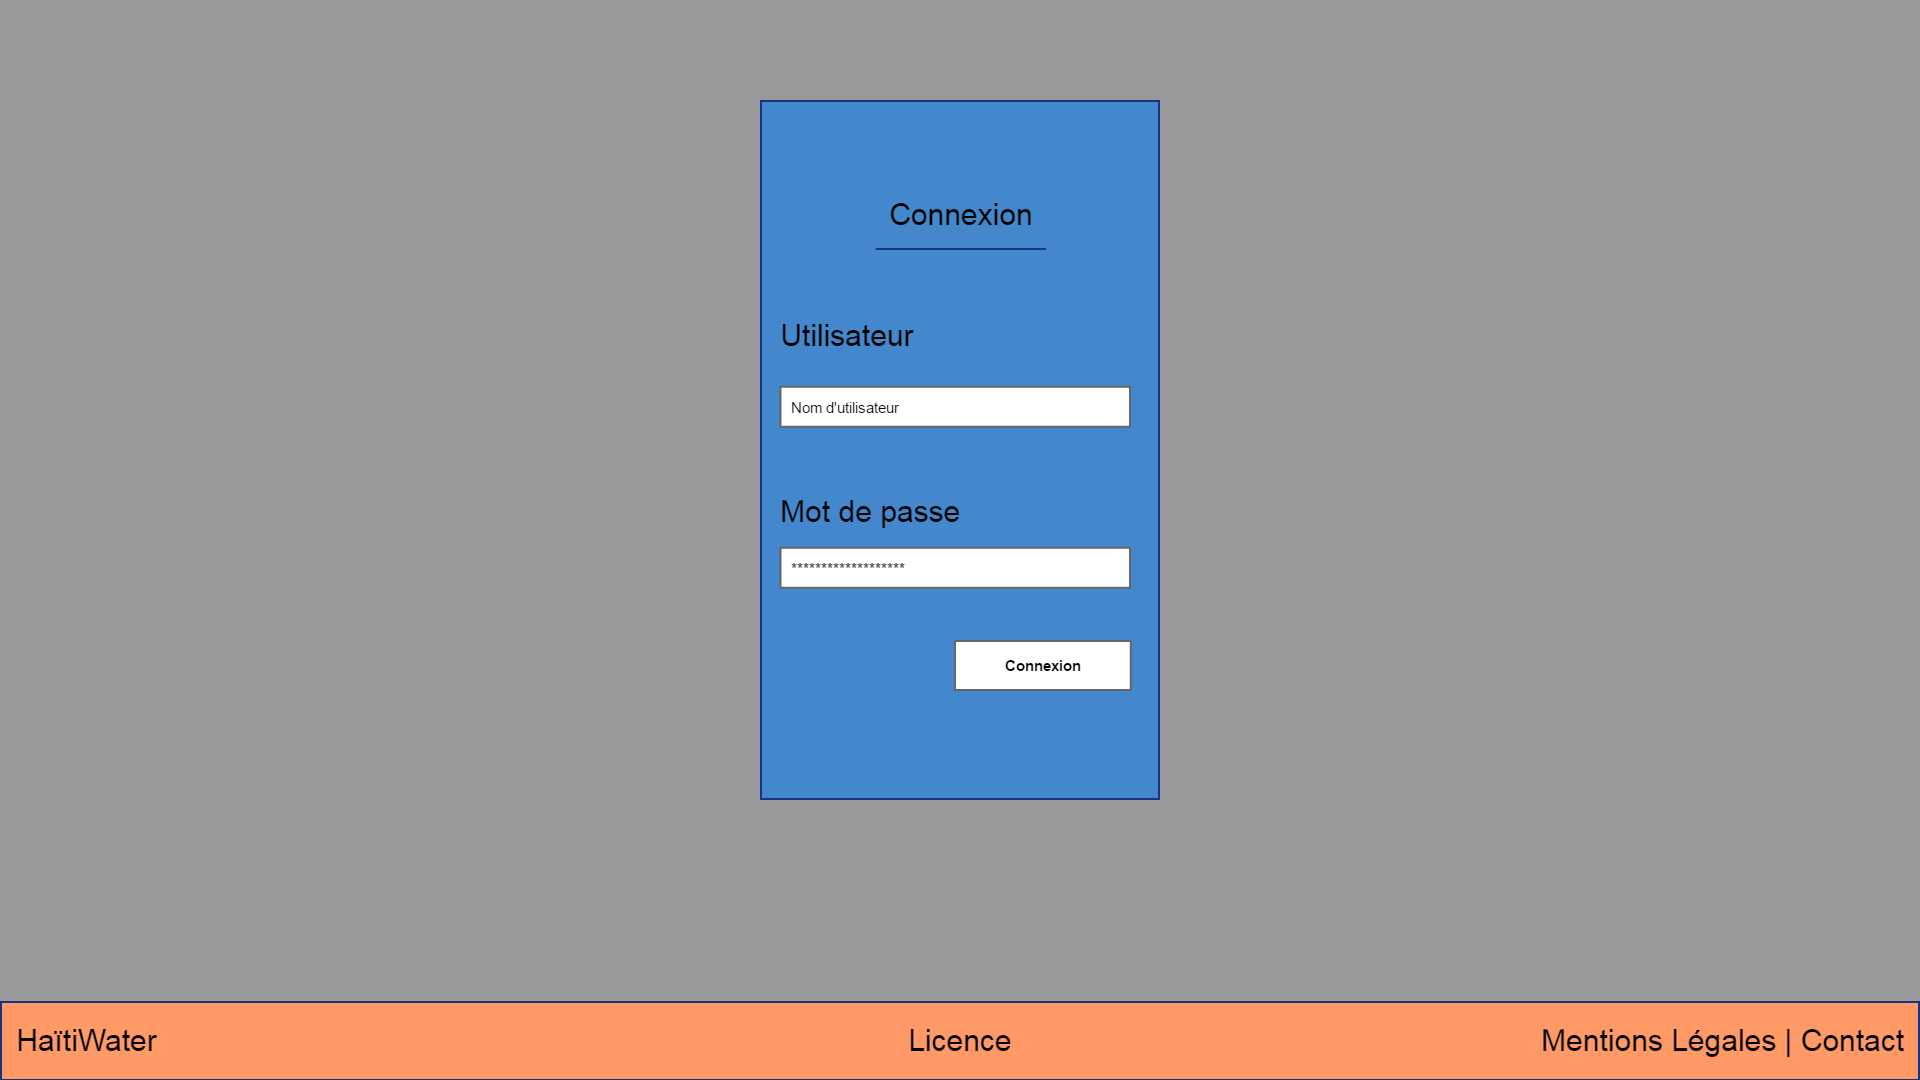
\includegraphics[width=\textwidth]{Cahier_des_Charges/login}
        \caption{\'Ecran d'identification}
        \label{fig:login}
    \end{figure}

    L'application fonctionne sur base des permissions de chaque utilisateur. La figure~\ref{fig:login} montre l'écran sur lequel tout utilisateur de l'application commence afin de pouvoir se connecter. Chaque utilisateur dispose au préalable de ses identifiants de connexion qui lui ont été fournis par sa hiérarchie.

    \begin{figure}[H]
        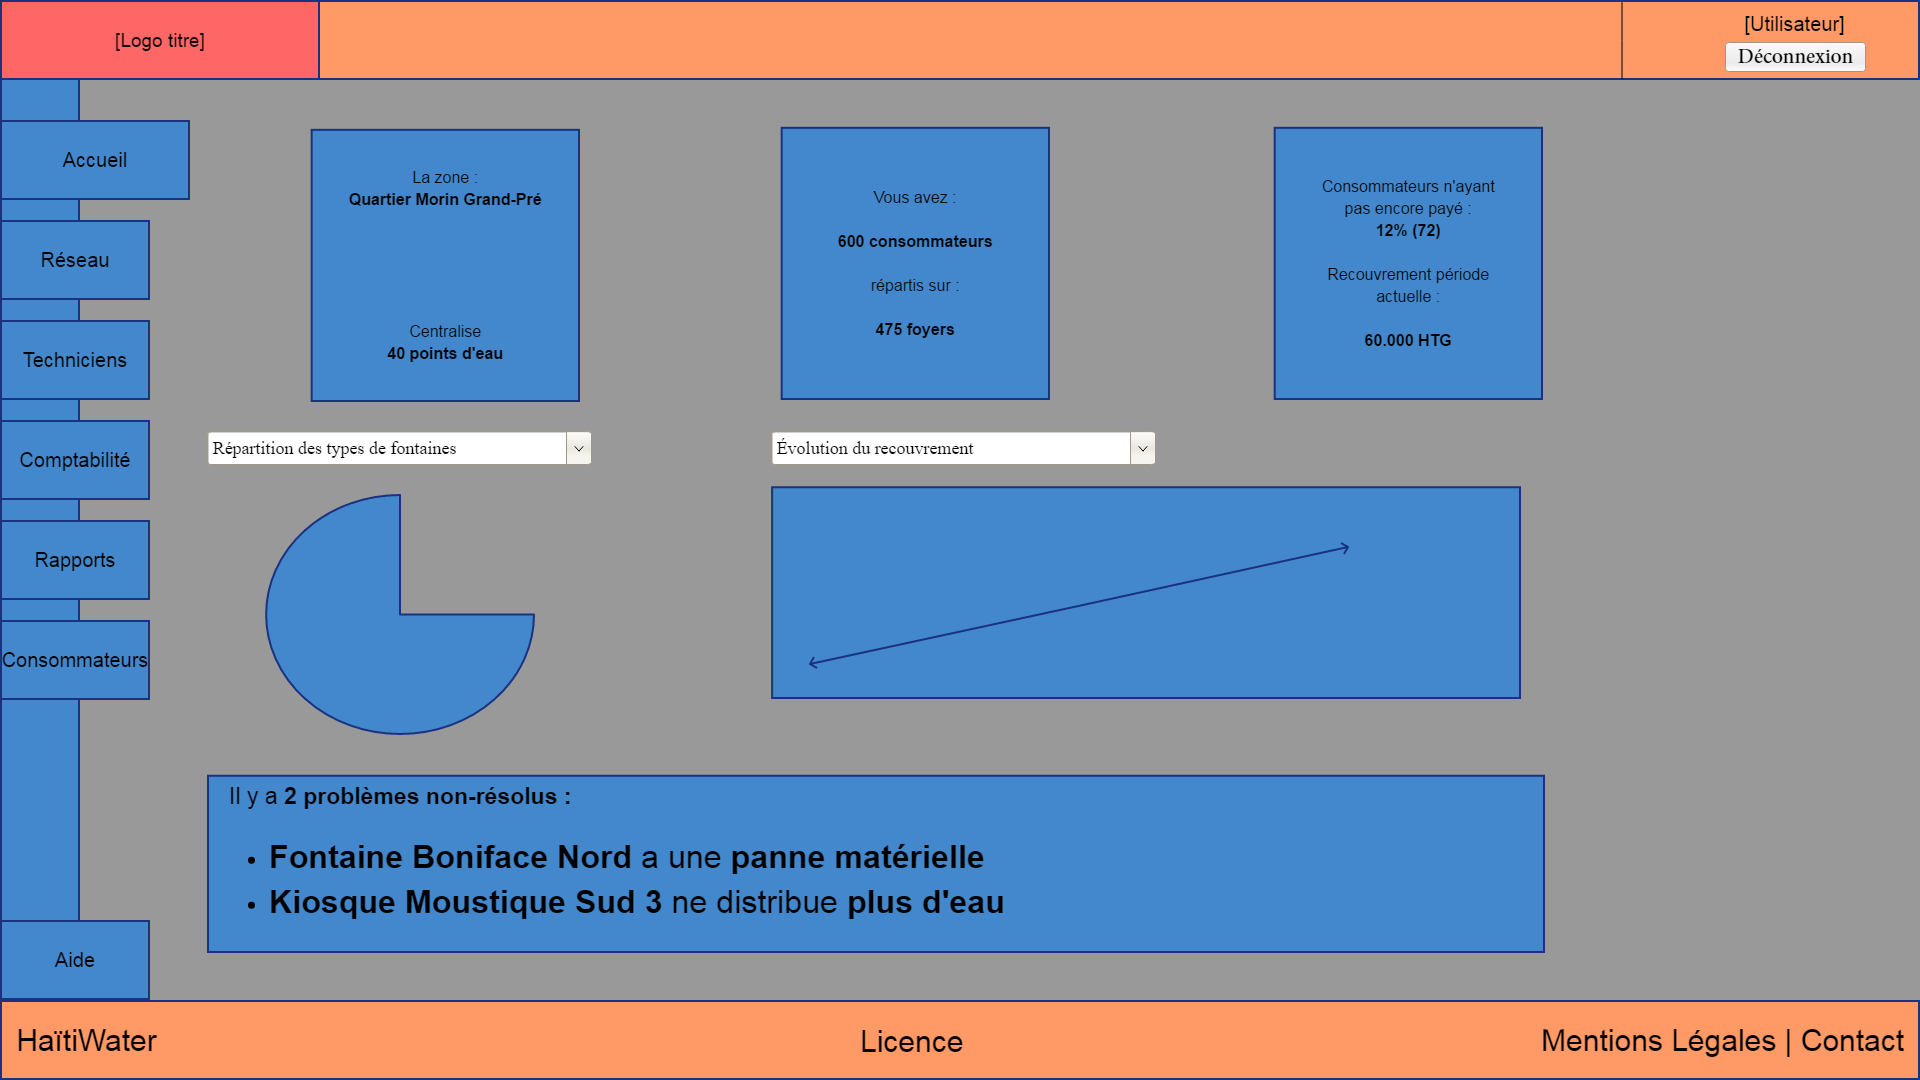
\includegraphics[width=\textwidth]{Cahier_des_Charges/accueil} % ToDo : modifier l'écran pour montrer un exemple
        \caption{\'Ecran d'accueil}
        \label{fig:dashboard}
    \end{figure}

    Une fois connecté, l'utilisateur dispose d'un écran d'accueil (figure~\ref{fig:dashboard}) personnalisé qui affiche des informations en fonction de son rôle. Un technicien voit la liste et le nombre des interventions en attente.
    \begin{description}
      \item[Un gestionnaire de zone et gestionnaire de fontaines] voient les sorties d'eau du réseau dont ils sont responsables (fontaines, réservoirs et prises individuelles) et leur état de fonctionnement (en service, hors service, en cours de réparation). Ils disposent également de statistiques mises en avant (quantité d'eau distribuée, somme des recettes, nombre d'utilisateurs) afin de proposer un accès rapide aux informations les plus importantes.\\
      Le gestionnaire de zone dispose en plus de la liste des gestionnaires de fontaines sous sa responsabilité.
      \item[Un technicien/plombier] voit le nombre et la liste des interventions en attente.
    \end{description}
    Sur la gauche, chaque utilisateur voit le menu comprenant les pages auxquelles il a accès. Tous les utilisateurs n'ont pas les mêmes permissions. Le gestionnaire de zone peut voir tous les menus permettant de gérer le réseau, les consommateurs, les techniciens, les gestionnaires de fontaine et problèmes qui sont sous sa responsabilité. Le gestionnaire de fontaine peut voir le réseau auquel il est assigné, les consommateurs et problèmes des points sous sa responsabilité.


  \subsection{Gestionnaire de fontaine}
  \begin{figure}[H]
      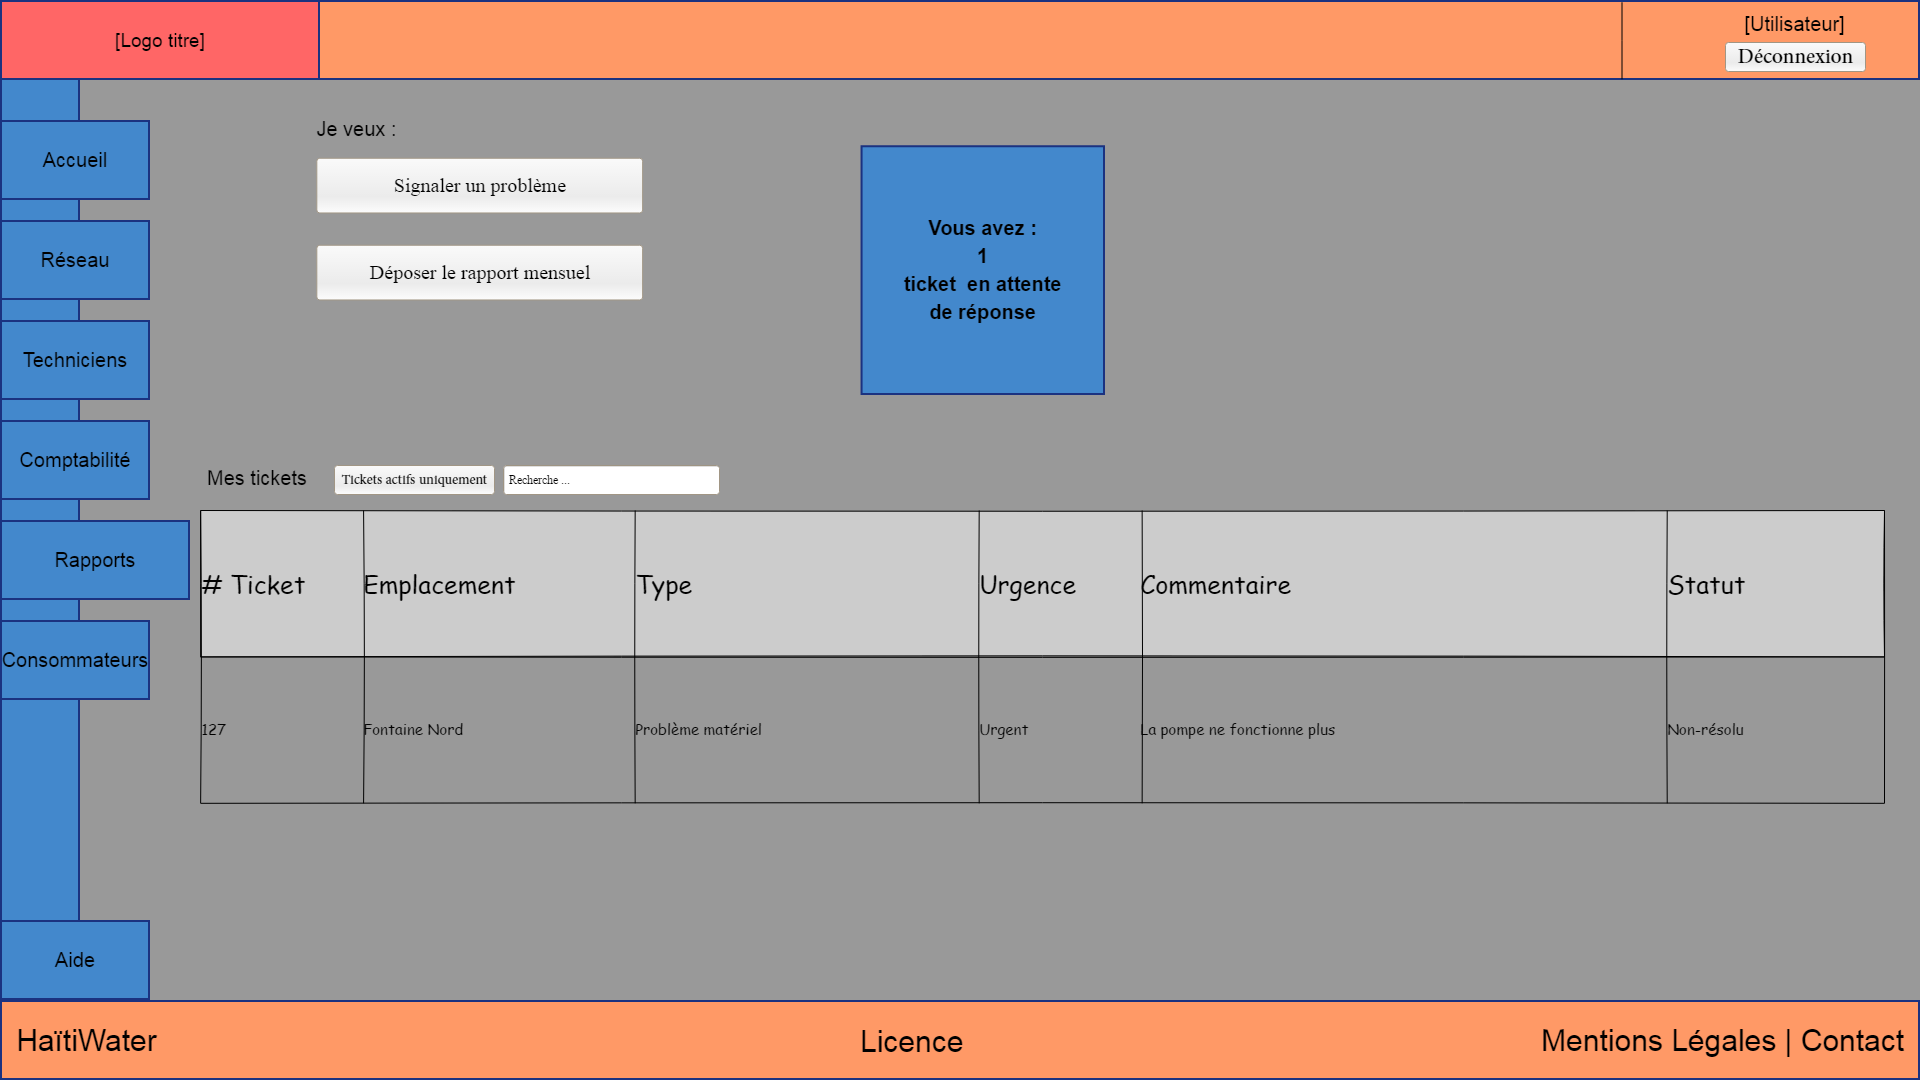
\includegraphics[width=\textwidth]{Cahier_des_Charges/rapports}
      \caption{Test}
      \label{fig:reports}
  \end{figure}

\section{Besoins non-fonctionnels}
% Explication des besoins non-fonctionnels
\section{Approche utilisée dans la création de ce document}
% D'où viennent les idées
% PS au lecteur : si vous voyez une autre source d'idées envoyez là !
\section{Choix technolgiques}
% Point de vue purement "positif pour le projet" sans termes techniques
\end{document}
